\begin{usecase}{02}{Autenticazione presso il sistema}
\usecaseprimaryactors{Utente non autenticato}
\usecasepre{L'utente ha avviato l'applicazione e ha selezionato la funzionalità di accesso nella schermata iniziale.}
\usecasedesc{L'utente può inserire il server a cui connettersi e le proprie credenziali per poter accedere presso il sistema.}
\usecasepost{L'utente si è autenticato presso il sistema.}
\usecaseext{UC02.5, UC02.6}
\label{uc:UC02}
\end{usecase}

\begin{figure}[!h] 
    \centering 
    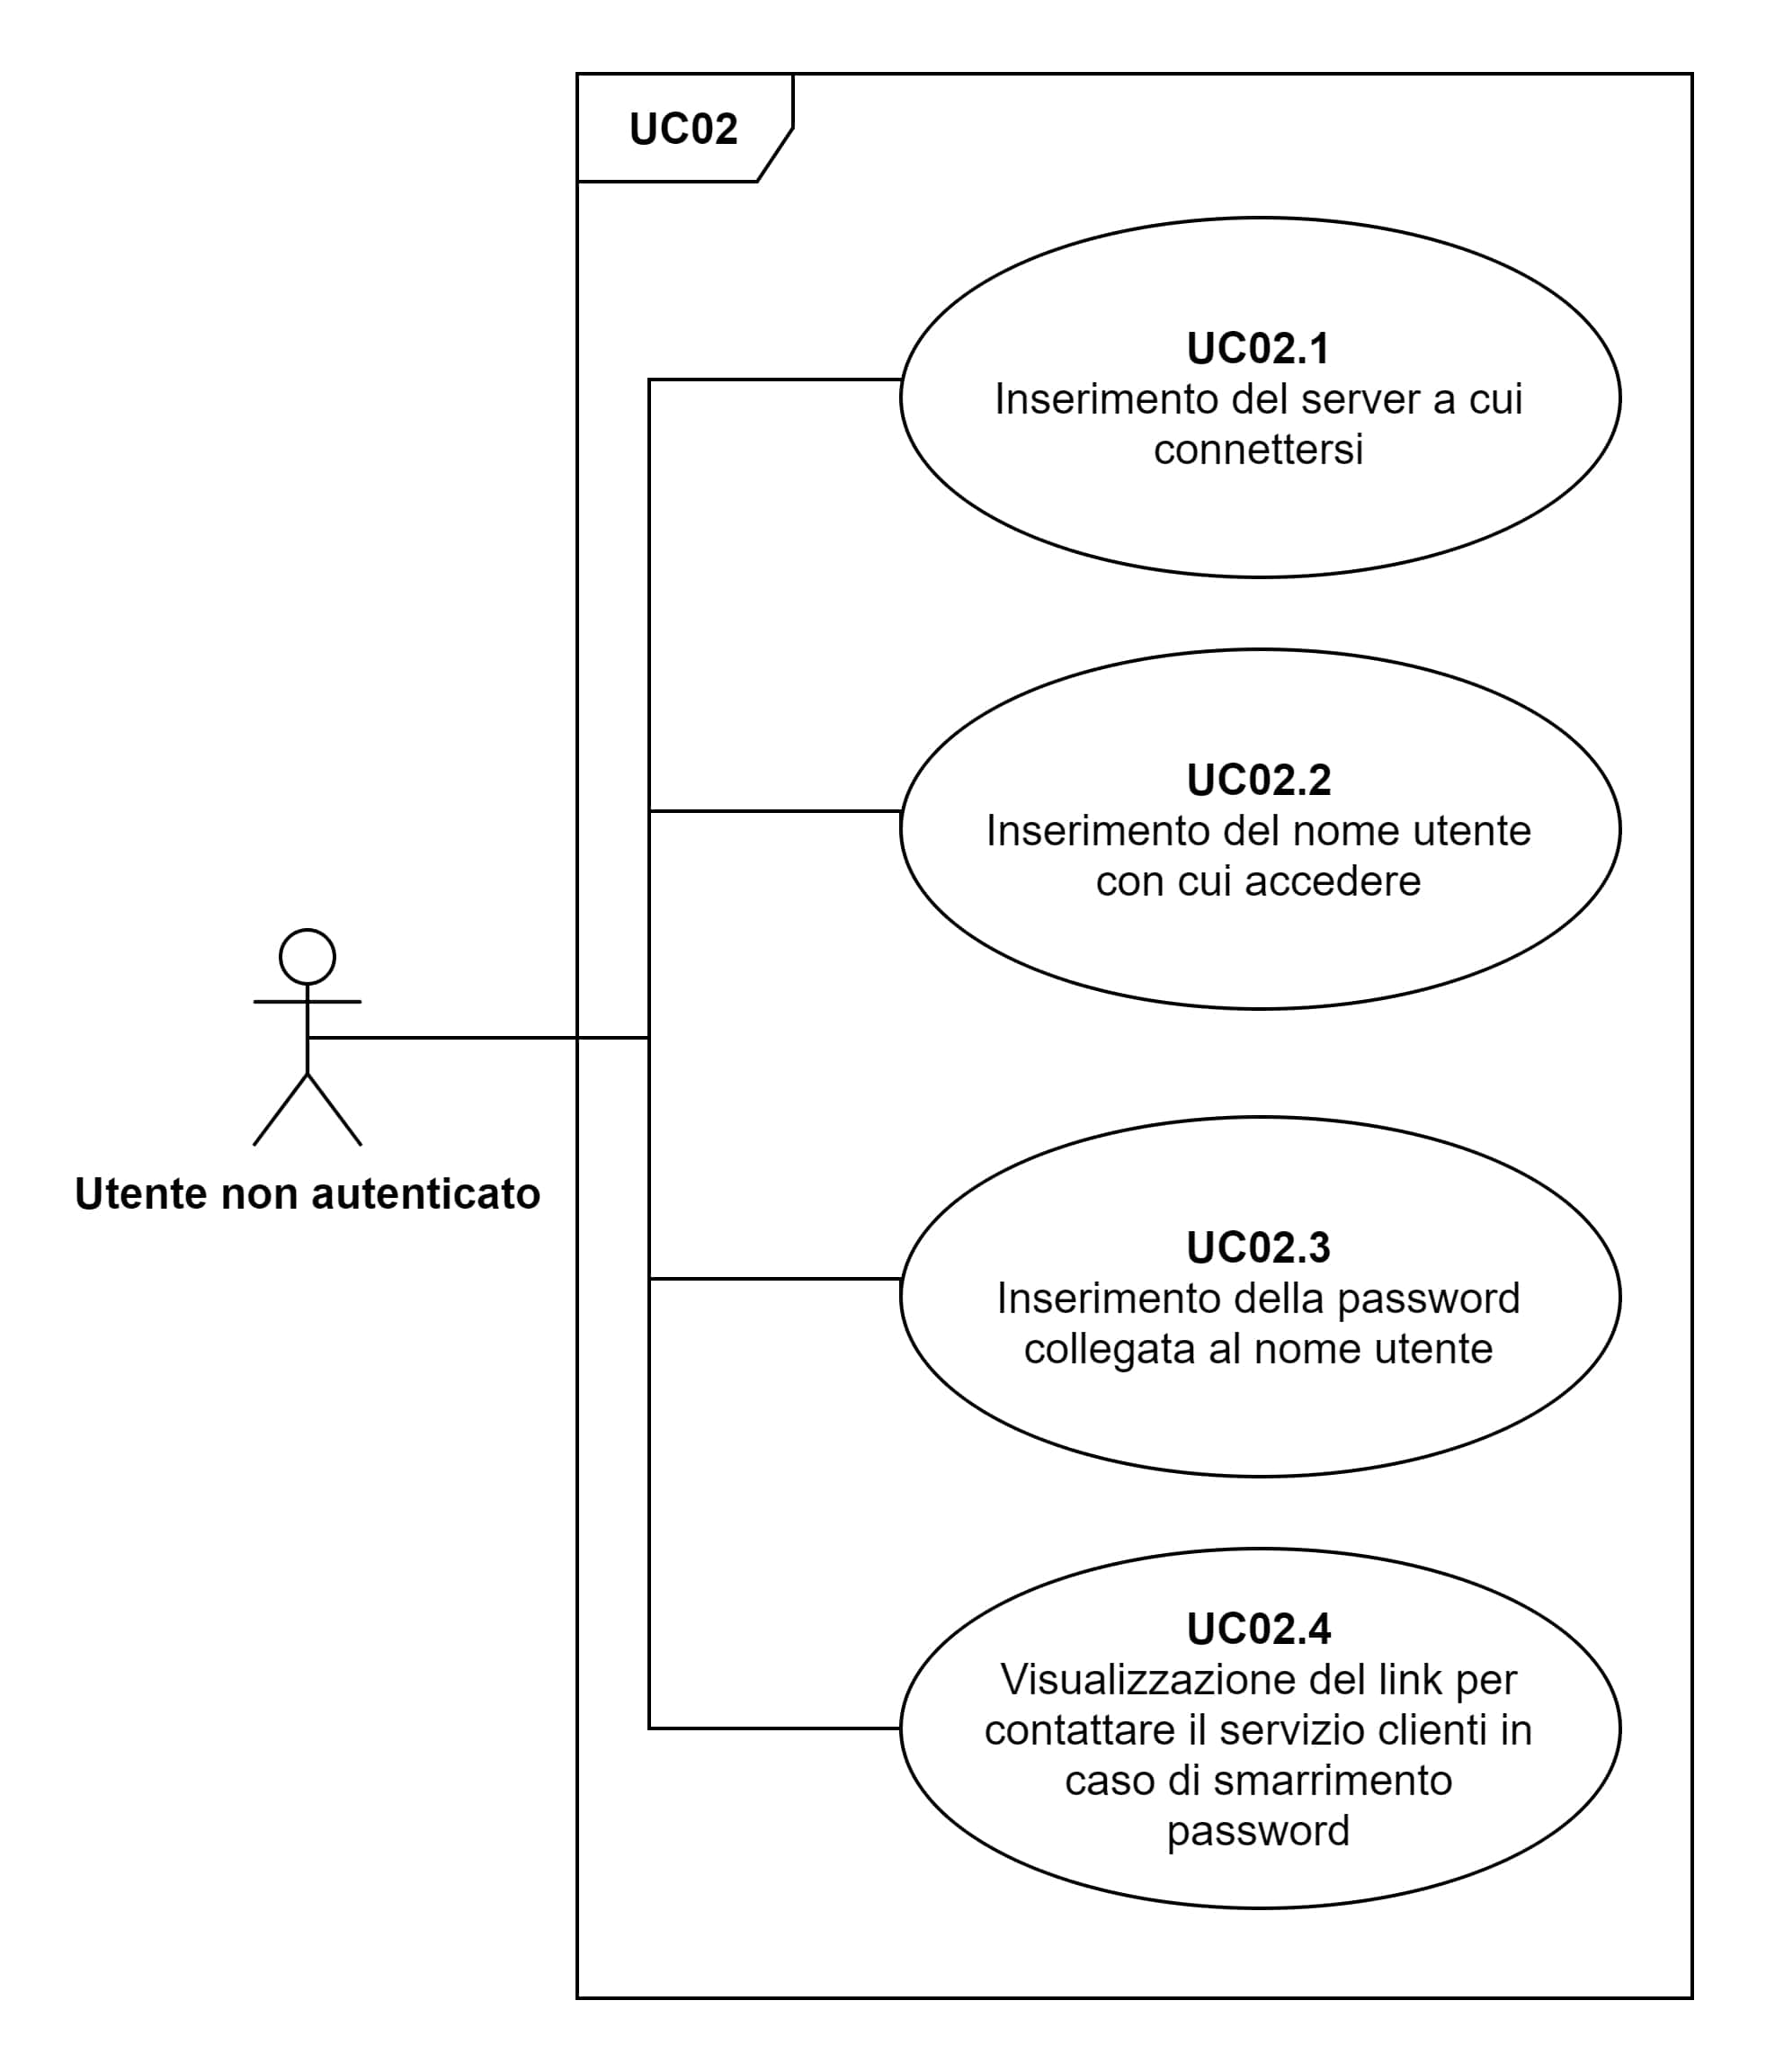
\includegraphics[width=1.0\columnwidth]{appendice-A/uc02} 
    \caption{SMacs - Sotto-casi d'uso di UC02 - Autenticazione presso il sistema}
\end{figure}

\begin{usecase}{02.1}{Inserimento del server a cui connettersi}
\usecaseprimaryactors{Utente non autenticato}
\usecasepre{L'utente ha la possibilità di inserire il server del sistema presso cui connettersi.}
\usecasedesc{L'utente può inserire il server a cui connettersi.}
\usecasepost{L'utente ha inserito il server a cui connettersi.}
\label{uc:UC02-1}
\end{usecase}

\begin{usecase}{02.2}{Inserimento del nome utente con cui accedere}
\usecaseprimaryactors{Utente non autenticato}
\usecasepre{L'utente ha la possibilità di inserire il nome utente con cui connettersi al sistema.}
\usecasedesc{L'utente può inserire il nome utente con cui connettersi al sistema.}
\usecasepost{L'utente ha inserito il proprio nome utente.}
\label{uc:UC02-2}
\end{usecase}

\begin{usecase}{02.3}{Inserimento della password collegata al nome utente}
\usecaseprimaryactors{Utente non autenticato}
\usecasepre{L'utente ha la possibilità di inserire la password con cui connettersi al sistema.}
\usecasedesc{L'utente può inserire la password con cui connettersi al sistema.}
\usecasepost{L'utente ha inserito la propria password.}
\label{uc:UC02-3}
\end{usecase}

\begin{usecase}{02.4}{Visualizzazione del link per contattare il servizio clienti in caso di smarrimento password}
\usecaseprimaryactors{Utente non autenticato}
\usecasepre{L'utente ha la possibilità di contattare il servizio clienti.}
\usecasedesc{L'utente può visualizzare il link per contattare il servizio clienti in caso di smarrimento della password.}
\usecasepost{Viene visualizzato il link per contattare il servizio clienti nel caso di smarrimento della password.}
\label{uc:UC02-4}
\end{usecase}

\begin{usecase}{02.5}{Visualizzazione messaggio di errore quando il server indicato è errato}
\usecaseprimaryactors{Utente non autenticato}
\usecasepre{L'utente ha inserito un server inesistente o a cui non è possibile connettersi.}
\usecasedesc{L'utente ha inserito un server inesistente o a cui non è possibile connettersi, di conseguenza viene visualizzato un messaggio di errore che lo informa del fatto.}
\usecasepost{Viene visualizzato un messaggio di errore che informa l'utente del fatto.}
\label{uc:UC02-5}
\end{usecase}

\begin{usecase}{02.6}{Visualizzazione messaggio di errore quando le credenziali inserite non sono valide}
\usecaseprimaryactors{Utente non autenticato}
\usecasepre{L'utente ha inserito delle credenziali errate.}
\usecasedesc{L'utente ha inserito delle credenziali errate e di conseguenza viene visualizzato un messaggio di errore che lo informa del fatto.}
\usecasepost{Viene visualizzato un messaggio di errore che informa l'utente del fatto.}
\label{uc:UC02-6}
\end{usecase}